\chapter{Refractory-Density and Age-Structured Population Methods}
\label{ch:refractory-density-age-structured}

\textit{Age-structured population theory keeps one microscopic fact that ordinary rate equations hide: neurons that just fired are different from neurons that have been silent for a long time. This matters for finite-size clustered networks because refractoriness and spike-history effects shape both the mean response and the noise.}

% ============================================================
\section{Age as time since last spike}
\label{sec:age-time-since-last-spike}
% ============================================================

For a spiking neuron, the most important history variable is often its \emph{age}: the time since its last spike. If neuron $i$ last fired at time $\hat t_i(t)$, define
%
\begin{equation}
  a_i(t)=t-\hat t_i(t).
  \label{eq:neuron-age}
\end{equation}
%
Between spikes, age increases at speed one:
%
\begin{equation}
  \dot a_i(t)=1.
  \label{eq:age-increase}
\end{equation}
%
When the neuron spikes, its age resets to zero:
%
\begin{equation}
  a_i(t^+)=0
  \qquad \text{if neuron } i \text{ spikes at } t.
  \label{eq:age-reset}
\end{equation}
%
Age is useful because it summarizes refractoriness. A neuron with $a_i=1$ ms may be unable or unlikely to spike, while a neuron with $a_i=100$ ms may be fully recovered. If adaptation currents also matter, age alone may be insufficient, but it is the first mesoscopic coordinate beyond a scalar rate.

For a population $\alpha$, the empirical age density is
%
\begin{equation}
  q_{\alpha,N}(a,t)
  =
  \frac{1}{N_\alpha}
  \sum_{i\in\alpha}\delta(a-a_i(t)).
  \label{eq:empirical-age-density}
\end{equation}
%
This density says what fraction of neurons in the population have age near $a$ at time $t$. It integrates to one:
%
\begin{equation}
  \int_0^\infty q_{\alpha,N}(a,t)\,\dd a=1.
  \label{eq:age-density-normalization}
\end{equation}
%
The scalar rate $R_\alpha(t)$ asks how many neurons are firing now. The density $q_\alpha(a,t)$ asks how ready the population is to fire in the near future.

% ============================================================
\section{Refractory-density equations}
\label{sec:refractory-density-equations}
% ============================================================

In the infinite-population limit, the empirical density is replaced by a smooth density $q_\alpha(a,t)$. Neurons move to larger age at speed one. They leave age $a$ when they spike. This gives the age-structured transport equation
%
\begin{keyequation}[Refractory-Density Equation]
\begin{equation}
  \pd{q_\alpha}{t}(a,t)
  +
  \pd{q_\alpha}{a}(a,t)
  =
  -\rho_\alpha(a,H_\alpha(t))\,q_\alpha(a,t),
  \qquad a>0 .
  \label{eq:refractory-density-pde}
\end{equation}
\tcblower
$q_\alpha(a,t)$: density of neurons with age $a$; \quad
$\partial_t q$: change in time; \quad
$\partial_a q$: drift toward older ages; \quad
$\rho_\alpha q_\alpha$: neurons leaving age $a$ by spiking.
\end{keyequation}

\noindent The function $\rho_\alpha(a,H_\alpha)$ is a hazard rate or escape intensity. It is the instantaneous probability per unit time that a neuron of age $a$ spikes under population input $H_\alpha$.

When neurons spike, they re-enter the density at age zero. The boundary condition is
%
\begin{equation}
  q_\alpha(0,t)=A_\alpha(t),
  \label{eq:age-density-boundary}
\end{equation}
%
where $A_\alpha(t)$ is the population activity. Activity is also obtained by integrating the hazard over the age density:
%
\begin{equation}
  A_\alpha(t)
  =
  \int_0^\infty
  \rho_\alpha(a,H_\alpha(t))\,q_\alpha(a,t)\,\dd a .
  \label{eq:activity-from-age-density}
\end{equation}
%
The boundary condition and the activity equation close the population dynamics. The same quantity $A_\alpha(t)$ is both the flux leaving the age density by spiking and the flux re-entering at age zero.

This is the key difference from an ordinary rate equation. A rate equation assumes the population has one state variable. The refractory-density equation keeps a distribution over recovery states.

\begin{figure}[h]
\centering
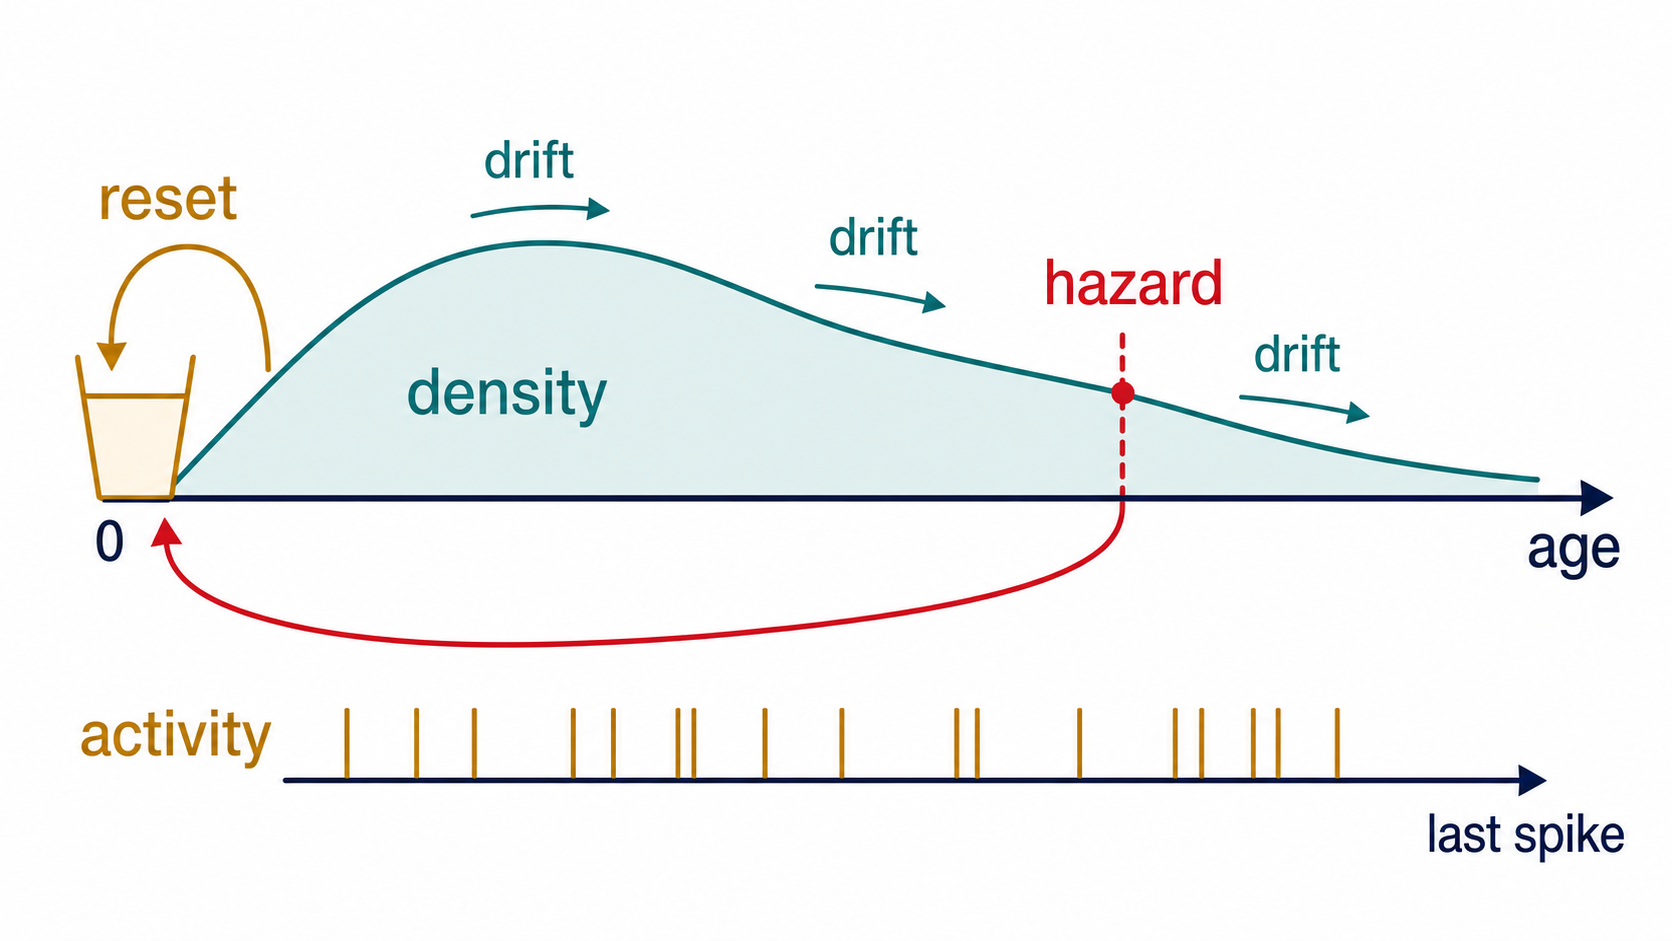
\includegraphics[width=0.95\textwidth]{figures/meso-refractory-density-flow.png}
\caption{Refractory-density theory replaces neuron identities by an age density over time since last spike. Probability mass drifts to larger ages, while the hazard selects part of the density to spike. Those spikes re-enter at age zero, and the reset flux is the population activity.}
\label{fig:refractory-density-flow}
\end{figure}

% ============================================================
\section{Survival functions and hazard rates}
\label{sec:survival-functions-hazard-rates}
% ============================================================

The hazard rate $\rho(a,H)$ is easier to interpret through the survival function. Suppose a neuron fired at time $t_0$ and has not fired again for age $a$. If the input trajectory is $H(t_0+s)$, the probability of surviving without a spike up to age $a$ is
%
\begin{equation}
  S(a\mid t_0)
  =
  \exp\!\left(
    -\int_0^a
    \rho(s,H(t_0+s))\,\dd s
  \right).
  \label{eq:survival-function-time-dependent}
\end{equation}
%
The integrand $\rho(s,H(t_0+s))$ is the instantaneous escape rate at age $s$. The integral accumulates escape risk. The exponential converts accumulated risk into survival probability.

For a stationary input $H$, the interspike-interval density is
%
\begin{equation}
  p_{\mathrm{ISI}}(a\mid H)
  =
  \rho(a,H)\,
  \exp\!\left(
    -\int_0^a \rho(s,H)\,\dd s
  \right).
  \label{eq:isi-density-hazard}
\end{equation}
%
The first factor says the neuron spikes at age $a$. The exponential says it did not spike before age $a$.

A hard absolute refractory period can be represented by
%
\begin{equation}
  \rho(a,H)=0
  \qquad
  \text{for } 0\le a<\tau_{\mathrm{ref}}.
  \label{eq:absolute-refractory-hazard}
\end{equation}
%
An escape-noise neuron can use a smooth hazard such as
%
\begin{equation}
  \rho(a,H)
  =
  c(a)\,
  \exp\!\left(\frac{u(H,a)-\vartheta}{\Delta_u}\right),
  \label{eq:escape-hazard-example}
\end{equation}
%
where $u(H,a)$ is an effective membrane drive, $\vartheta$ is threshold, $\Delta_u$ controls spike stochasticity, and $c(a)$ suppresses firing during refractoriness. This is not meant as the only possible hazard; it shows how membrane state, threshold, and refractoriness can enter the same population equation.

% ============================================================
\section{Renewal equations for population activity}
\label{sec:renewal-equations-population-activity}
% ============================================================

The age-density PDE can be rewritten as a renewal equation. Every neuron firing at time $t$ must have fired previously at time $t-a$ and then survived for age $a$ before firing again.

For a homogeneous renewal population without initial-condition terms, the activity satisfies
%
\begin{equation}
  A(t)
  =
  \int_0^\infty
  A(t-a)\,
  p_{\mathrm{ISI}}(a\mid t-a)\,
  \dd a,
  \label{eq:renewal-equation-activity}
\end{equation}
%
where
%
\begin{equation}
  p_{\mathrm{ISI}}(a\mid t-a)
  =
  \rho(a,H(t))\,
  \exp\!\left(
    -\int_0^a
    \rho(s,H(t-a+s))\,\dd s
  \right).
  \label{eq:time-dependent-isi-kernel}
\end{equation}
%
The factor $A(t-a)\,\dd a$ is the fraction of neurons whose previous spike occurred in a small interval around $t-a$. The kernel is the probability density that their next spike occurs exactly $a$ later.

For constant input, the stationary firing rate is the reciprocal of the mean ISI:
%
\begin{equation}
  r(H)
  =
  \frac{1}{
    \int_0^\infty a\,p_{\mathrm{ISI}}(a\mid H)\,\dd a
  }.
  \label{eq:stationary-rate-from-isi}
\end{equation}
%
This equation defines a transfer function from the hazard model. It connects the age-structured description back to the mean-field transfer function:
%
\begin{equation}
  \Phi(H)=r(H).
  \label{eq:transfer-from-renewal}
\end{equation}
%
The renewal view is useful when spike-history effects matter strongly. Instead of assuming the population rate instantly follows $\Phi(H)$, it computes how the current age distribution constrains the next activity pulse.

% ============================================================
\section{Finite-size refractory-density models}
\label{sec:finite-size-refractory-density-models}
% ============================================================

In a finite population, the age density is not smooth. It is the empirical measure from \cref{eq:empirical-age-density}. The finite-size population activity is a random flux through the spiking boundary:
%
\begin{equation}
  A_{\alpha,N}(t)
  =
  \frac{1}{N_\alpha}\sum_{i\in\alpha}X_i(t).
  \label{eq:finite-size-population-activity-age}
\end{equation}
%
A compact stochastic age-density model is
%
\begin{align}
  \pd{q_{\alpha,N}}{t}
  +
  \pd{q_{\alpha,N}}{a}
  &=
  -\rho_\alpha(a,H_\alpha(t))q_{\alpha,N}(a,t)
  + A_{\alpha,N}(t)\delta(a),
  \label{eq:finite-size-age-density-delta}
  \\
  A_{\alpha,N}(t)
  &=
  \int_0^\infty
  \rho_\alpha(a,H_\alpha(t))q_{\alpha,N}(a,t)\,\dd a
  +
  \frac{1}{\sqrt{N_\alpha}}\eta_\alpha(t).
  \label{eq:finite-size-age-activity-noise}
\end{align}
%
The delta source at $a=0$ resets spiking neurons to age zero. The noise term $\eta_\alpha$ represents the difference between expected spike flux and realized spike flux in a finite population.

In a small time bin $\Delta t$, conditional on the current density, the expected spike fraction is approximately
%
\begin{equation}
  \E[\Delta n_\alpha\mid q_{\alpha,N}]
  =
  \Delta t
  \int_0^\infty
  \rho_\alpha(a,H_\alpha(t))q_{\alpha,N}(a,t)\,\dd a,
  \label{eq:expected-spike-fraction-age}
\end{equation}
%
and the variance is approximately
%
\begin{equation}
  \Var[\Delta n_\alpha\mid q_{\alpha,N}]
  \approx
  \frac{\Delta t}{N_\alpha}
  \int_0^\infty
  \rho_\alpha(a,H_\alpha(t))q_{\alpha,N}(a,t)\,\dd a,
  \label{eq:variance-spike-fraction-age}
\end{equation}
%
when individual spikes are conditionally independent in that bin. This again gives the $N_\alpha^{-1/2}$ scaling.

The subtle point is that refractory-density noise is not only white counting noise. A large activity fluctuation at time $t$ changes the age density by putting many neurons at age zero. That altered density changes the probability of spikes in the future. Thus finite-size fluctuations can be temporally structured even when the underlying spike decisions are conditionally independent.

% ============================================================
\section{Connection to Schwalger, Deger, and Gerstner 2017}
\label{sec:connection-schwalger-deger-gerstner}
% ============================================================

\textbf{Citation TODO for coordinator.} This section should be connected to the Schwalger, Deger, and Gerstner mesoscopic population framework, commonly cited for finite-size population equations for generalized integrate-and-fire neurons. The exact bibliography key should be resolved by the final coordinator rather than guessed here.

The relevant conceptual bridge is this: generalized integrate-and-fire neurons can often be described by a hazard that depends on input and spike history. In an infinite population, the refractory-density or renewal equation gives the deterministic population activity. In a finite population, the realized activity fluctuates around that deterministic value with a noise term whose amplitude and temporal structure are determined by the finite number of neurons.

A schematic version of the finite-size population activity equation is
%
\begin{equation}
  A_N(t)
  =
  A_\infty(t)
  +
  \frac{1}{\sqrt{N}}\,
  \zeta(t),
  \label{eq:sdg-schematic-finite-size}
\end{equation}
%
where $A_\infty(t)$ is the activity predicted by the infinite-population age-density equation and $\zeta(t)$ is a stochastic fluctuation process. The important claim is not merely that noise scales like $N^{-1/2}$. The noise must be consistent with renewal structure: a fluctuation in spike count changes the future refractory pool.

For clustered networks, this matters because each cluster may contain only hundreds or thousands of neurons, not an infinite population. A mesoscopic theory that treats cluster activity as deterministic until arbitrary external noise is added misses the renewal constraint. A theory derived from finite-size population equations keeps that constraint.

% ============================================================
\section{Why this framework is relevant to clustered networks}
\label{sec:why-age-framework-relevant-clustered}
% ============================================================

Clustered networks are usually discussed in terms of attractors, but transitions between attractors occur through spikes. Refractory-density theory supplies a bridge between spike-history mechanisms and cluster-level state variables.

Consider an excitatory cluster in an up-state. Its recurrent input is high, so its hazard is high. But high recent activity also fills the refractory part of the age density. The next activity pulse depends on both the input and the number of neurons that are available to fire:
%
\begin{equation}
  A_\alpha(t)
  =
  \int_0^\infty
  \rho_\alpha(a,H_\alpha(t))q_\alpha(a,t)\,\dd a.
  \label{eq:cluster-activity-availability}
\end{equation}
%
The input $H_\alpha$ measures drive. The density $q_\alpha$ measures availability. Both are needed. A cluster with strong input but many refractory neurons may transiently fire less than a memoryless rate model predicts.

This is especially relevant for E/I-clustered networks. Local inhibitory activity can rapidly reduce excitatory hazard, while excitatory refractory depletion can slow subsequent excitation. The mesoscopic state may therefore need at least
%
\begin{equation}
  \left(q_{\alpha E}(a,t),\,q_{\alpha I}(a,t),\,H_{\alpha E}(t),\,H_{\alpha I}(t)\right)
  \label{eq:ei-age-state}
\end{equation}
%
or a reduced set of moments derived from these densities. A scalar excitatory rate may not capture the timing relation between local excitation, local inhibition, and recovery from refractoriness.

For metastability, the age-density framework also predicts how switching statistics should change with cluster size. If escape is caused by finite-size population fluctuations, the noise amplitude should shrink as $N_\alpha^{-1/2}$ and dwell times should increase. If escape is caused by deterministic mesoscopic instability, the age-density noise may modulate switching but should not be the primary scaling law.

% ============================================================
\section{How to read Tilo's mesoscopic equations}
\label{sec:how-to-read-tilos-mesoscopic-equations}
% ============================================================

When reading mesoscopic equations from Tilo's work or related population-density papers, separate the notation into four layers.

First, identify the activity variable. It is often written as $A(t)$, $\nu(t)$, or $r(t)$. This is the population spike flux: spikes per neuron per unit time.

Second, identify the hidden population state. In an age-structured formulation this is $q(a,t)$ or a related refractory density. In a quasi-renewal approximation it may be represented through filtered activity traces rather than a full density.

Third, identify the hazard or gain. This is the map from input and history to spike probability:
%
\begin{equation}
  \rho(t,a)
  =
  \rho\!\left(a, H(t), \text{history variables}\right).
  \label{eq:reading-hazard}
\end{equation}
%
If the hazard depends strongly on age, the population has memory even if the input $H(t)$ is fixed.

Fourth, identify the finite-size term. A useful schematic reading is
%
\begin{equation}
  \text{population activity}
  =
  \text{deterministic renewal prediction}
  +
  \text{finite-size fluctuation}.
  \label{eq:reading-finite-size-term}
\end{equation}
%
The fluctuation is not arbitrary measurement noise. It is the stochastic error made when $N$ neurons sample the hazard. Its amplitude, covariance, and future consequences are constrained by the population state.

For this rotation, the reading goal is concrete. Translate each term into one of the following: input drive, spike-history availability, deterministic population flux, recurrent coupling, or finite-size fluctuation. Once every term has one of these roles, the equations become a candidate mesoscopic theory for each cluster.

\begin{chaptersummary}

\begin{center}
\renewcommand{\arraystretch}{1.55}
\begin{tabularx}{\textwidth}{@{}l X X@{}}
  \toprule
  \textbf{Object} & \textbf{Equation} & \textbf{Meaning} \\
  \midrule
  Age &
  $a_i(t)=t-\hat t_i(t)$ &
  Time since neuron $i$ last fired \\
  Age density &
  $q_N(a,t)=N^{-1}\sum_i\delta(a-a_i(t))$ &
  Fraction of neurons with recovery age $a$ \\
  Refractory-density PDE &
  $\partial_t q+\partial_a q=-\rho q$ &
  Neurons age and leave by spiking \\
  Boundary flux &
  $q(0,t)=A(t)$ &
  Spikes reset neurons to age zero \\
  Activity &
  $A(t)=\int\rho(a,H(t))q(a,t)\,\dd a$ &
  Hazard averaged over available neurons \\
  Renewal kernel &
  $p_{\mathrm{ISI}}(a)=\rho(a)S(a)$ &
  Spike at age $a$ after surviving earlier ages \\
  Finite-size scaling &
  $A_N=A_\infty+N^{-1/2}\zeta$ &
  Population spike flux fluctuates because $N$ is finite \\
  \bottomrule
\end{tabularx}
\end{center}

\end{chaptersummary}

\begin{conceptquestions}
  \item What information does the age density contain that a scalar firing rate does not?
  \item In the refractory-density PDE, why does the term $\partial_a q$ appear with coefficient one?
  \item Explain why the same activity $A(t)$ appears both as an integral over hazards and as the boundary condition at age zero.
  \item Derive the ISI density $p_{\mathrm{ISI}}(a)=\rho(a)S(a)$ from the survival function.
  \item Why can a large finite-size spike-count fluctuation affect future activity even after the instantaneous noise has passed?
  \item For an E/I-clustered model, why might one need separate age densities for excitatory and inhibitory subpopulations?
  \item When reading a finite-size mesoscopic population equation, how would you identify which term represents deterministic flux and which term represents finite-size sampling?
\end{conceptquestions}
